\documentclass[11pt]{beamer}





\usepackage{lmodern} 		% Diese beiden packages sorgen für echte 
\usepackage[T1]{fontenc}	% Umlaute.

\usepackage{amssymb, amsmath, color, graphicx, float, setspace, tipa}
\usepackage[utf8]{inputenc} 
\usepackage[english]{babel}
\usepackage[justification=centering]{caption}
\addto\captionsenglish{\renewcommand{\figurename}{}} %Abbildungen nicht bzw. anders beschriften.


%\usepackage[pdfpagelabels,pdfstartview = FitH,bookmarksopen = true,bookmarksnumbered = true,linkcolor = black,plainpages = false,hypertexnames = false,citecolor = black, breaklinks]{hyperref}
%\usepackage{url}
\usepackage{picins} 		%Gleittext um Grafik. Befehl: parpic. Vorlage siehe unten
\usepackage{longtable} 		%Seitenübergreifende Tabelle. Vorlage siehe unten
\newtheorem*{bem}{Bemerkung} % Neue Theorem-Umgebung: Bemerkung
\newcommand{\fillframe}{\vskip0pt plus 1filll} 
\newcommand{\musr}{$\mu$SR }


%-----------------
%BEAMER-SPEZIFISCH
%-----------------

\usetheme{default}
% Verschiedene Varianten von usetheme, usecolortheme und usefonttheme kann man hier ausprobieren: http://deic.uab.es/~iblanes/beamer_gallery/

% \usetheme{
% 	AnnArbor | Antibes | Bergen |
% 	Berkeley | Berlin | Boadilla |
% 	boxes | CambridgeUS | Copenhagen |
% 	Darmstadt | default | Dresden |
% 	Frankfurt | Goettingen |Hannover |
% 	Ilmenau | JuanLesPins | Luebeck |
% 	Madrid | Malmoe | Marburg |
% 	Montpellier | PaloAlto | Pittsburgh |
% 	Rochester | Singapore | Szeged |
% 	Warsaw
% }
%Interessant scheinen: Boadilla, boxes, CambridgeUS, default, (Goettingen), Hannover, Madrid, Montpellier, Pittsburgh, Rochester, Singapore, Szeged, 

\usecolortheme{dove}
% \usecolortheme{
% 	albatross | beaver | beetle |
% 	crane | default | dolphin |
% 	dove | fly | lily | orchid |
% 	rose |seagull | seahorse |
% 	sidebartab | structure |
% 	whale | wolverine
% }

\usefonttheme{structurebold}
% 	default | professionalfonts | serif |
% 	structurebold | structureitalicserif |
% 	structuresmallcapsserif
% }


%\useinnertheme{
% 	circles | default | inmargin |
% 	rectangles | rounded
% } Am besten sein lassen.


% \useoutertheme{
% 	default | infolines | miniframes |
% 	shadow | sidebar | smoothbars |
% 	smoothtree | split | tree
% } Am besten sein lassen.



\setbeamercovered{transparent} %Halbtransparente Overlays (was als nächstes Element auf der Folie gezeigt wird)
\beamertemplatenavigationsymbolsempty % Entfernt Navigationssymbole unten
%\setbeamertemplate{footline}[frame]  % Seitenzahlen
    \setbeamertemplate{footline}{%
    	\raisebox{5pt}{\makebox[\paperwidth]{\hfill\makebox[10pt]{\hyperlink{tableofcontents}{\scriptsize\insertframenumber}}}}}



%---------------------
%--Metainformationen--
%---------------------
\title{Probing magnetic fields in solids using muon spin rotation}

\author[M. Ivkovic]{
	Mladen Ivkovic
}
\date[16.11.15]{16. November 2015}


% \title[Kurzform]{Vortrag zur Berechenbarkeit}
%     Titel des Vortrages
% \subtitle[Kurzform]{Untertitel}
%     Untertitel
% \author[M. Schulz]{Michael Schulz}
%     Autor festlegen
% \institute[IfI -- HU Berlin]{Institut für Informatik\\ Humboldt-Universität zu Berlin}
%     Angabe des Institutes
% \date[26.05.06]{26. Mai 2006}
%     Datum der Präsentation, alternativ kann mittels \date{\today} auch das aktuelle Datum eingetragen werden.
% \logo{\pgfimage[width=2cm,height=2cm]{hulogo}}
%     Die Datei hulogo.pdf (bzw. hulogo.png, hulogo.jpg, hulogo.mps bei Verwendung von pdftex als Backend) als Logo auf allen Folien, hier mithilfe des Paketes pgf.
% \titlegraphic{\includegraphics[width=2cm,height=2cm]{hulogo}}
%     Die Datei hulogo.pdf (bzw. analog wie bei \logo auch entsprechendes Format) als Logo nur auf der Titelseite unter Verwendung des Paketes graphicx.


%------------------------------------------------------------------
%------------------------------------------------------------------
%----------------VORLAGEN------------------------------------------
%----------------VORLAGEN------------------------------------------
%----------------VORLAGEN------------------------------------------
%------------------------------------------------------------------

%Bruch: \frac{}{}
%Kleiner Bruch: \tfrac{}{}
%Gleichungen: \begin{align}
%Delta für partielle Ableitungen: \partial
%Schönes Epsilon: \varepsilon

%Strich: in align-Umgebung, \bar{} oder \overline{}
%Seitenumbruch: \clearpage ; Besser als \newpage, da er floats zwingt, zuerst eingefügt zu werden.
%Zu grosse Zeilenabstände wegen Formelzeichen? -> \vphantom{}, \smash{}
%\newcommand{\BefehlName}[Anzahl_Parameter]{Definitiere neuen Befehl. Den ersten Parameter ruft man mit #1 ab, den zweiten mit #2 etc}

%%FIGUR
%\begin{figure}[htbp]
%\centering
%\includegraphics[width=15cm]{Bild1}%
%\caption{Experimental set-up}%
%\label{1}
%\end{figure}

%%BILD MIT PICINS NEBEN TEXT SETZEN
%\piccaption{Caption\label{label}} 
%\parpic[r]{\fbox{\includegraphics [width=5cm, keepaspectratio]{bild.png}}}
%


%% ZWEI BILDER NEBENEINANDER.
%% Schau, dass die minipages insgesamt nie mehr als 1.0\textwidth haben.
%% Um ein drittes oder viertes Bild einzufügen, ergänze einfach um weitere minipages.
% \begin{figure}[!htb]
% \centering
%   \minipage{0.3\textwidth}
%     \fbox{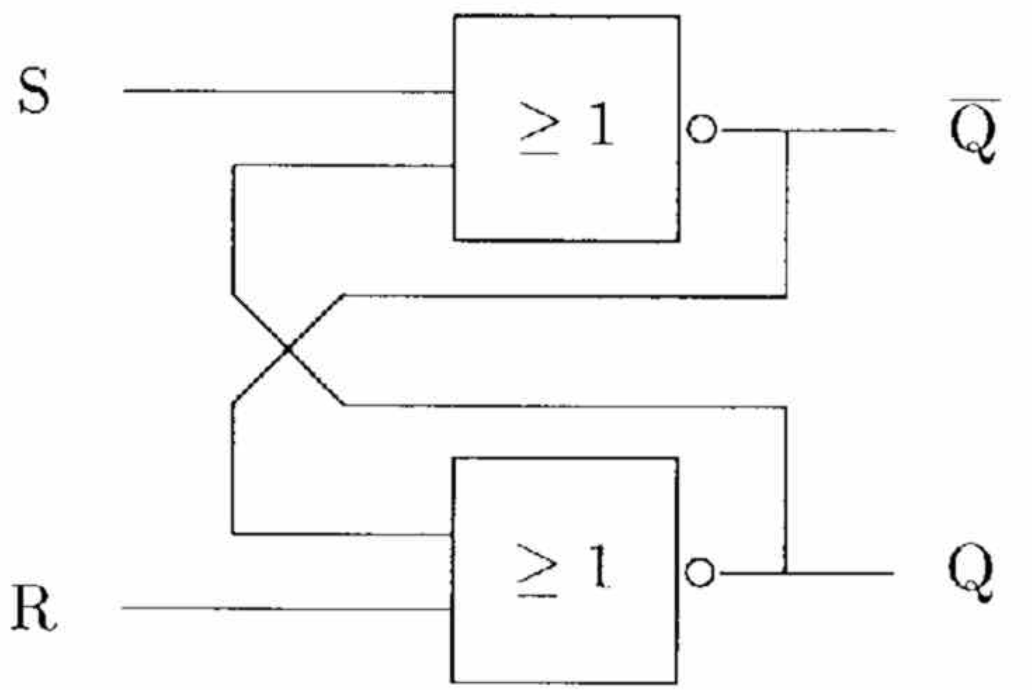
\includegraphics[height=2.5cm, keepaspectratio]{rsflipflop.png}}%
%     \caption{RS-Flipflop}%
%     \label{fig:rsflipflop}
%   \endminipage\hspace{1cm}   
% %
%   \minipage{0.4\textwidth}
%     \fbox{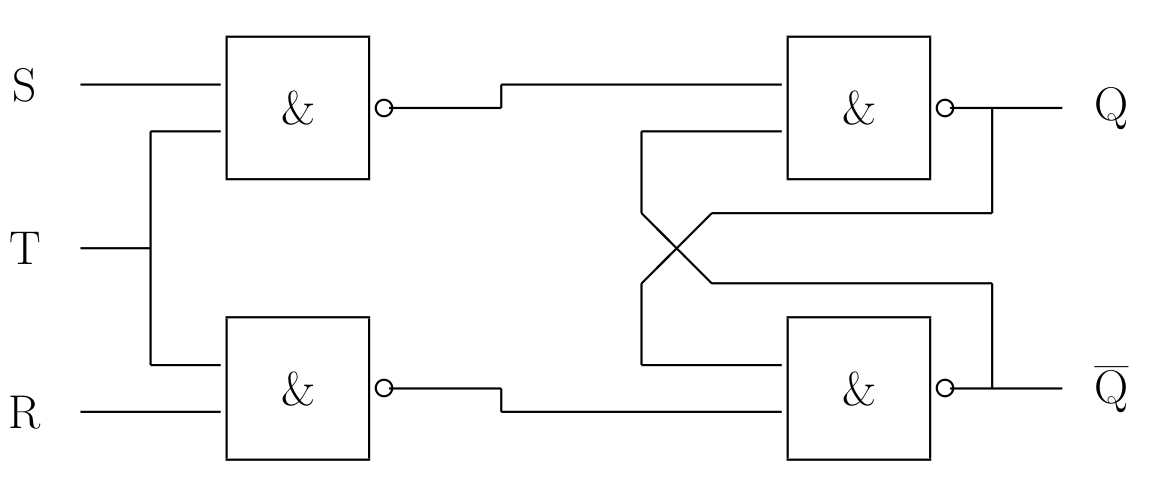
\includegraphics[height=2.5cm, keepaspectratio]{rsflipfloptakt.png}}%
%     \caption{getaktetes RS-Flipflop}%
%     \label{fig:rsflipfloptakt}
%   \endminipage
% \end{figure}



%% TABELLEN
%% 1) mit tabular
%\begin{center}
%\begin{tabular}[c]{|p{1cm}|p{3cm}|p{3cm}|p{3cm}|}
%\hline
%\multicolumn{2}{|c||}{Stromstärke 0.4A}	&	\multicolumn{2}{c|}{Stromstärke 0.6A}\\
%\hline
%$4T$ in s	&	$T'$		&	$4T$ in s	&	$T'$\\
%\hline
%7.1			&	1.775	&	7.1		& 	1.775\\
%\hline
%7.2			&	1.8		&	7.1		&	1.775\\
%\hline
%7.3			&	1.825	&	7.1		&	1.775\\
%\hline
%\end{tabular}
%\end{center}
%
%% 2) Mit longtable
%\begin{longtable}{p{3.5cm} p{11.5cm}}
%  Blabla & Blabla\\ [2mm] <= Macht 2mm Abstand zwischen Zeilen
%  %
%  Blabla & Blabla \\ [2mm]
%\end{longtable}


%%%%%%%%%%%%%%%%%%%%%%%%%%%%%%%%%%%%%%%%%%%%%%%%%%%%%%%%%%%%%%%%%%%%%%%%%%%%%%%%%%%%%%%%%%%%%%%%%%%%%%%%%%%%%%%%%%%%%%%%%%%%%%%%%%%%%%%%%%%%%%%%%%%%%%%%%%%%%%%%%%%%%%%%%%%%






\begin{document}

% \begin{frame}[Overlay-Aktionen][Optionen]{Titel}{Untertitel}
% 
% Overlay-Aktionen
%     Overlay-Aktionen setzen die Standard-Overlay-Aktionen aller Umgebungen innerhalb des Frames, welche Aktion-Spezifikationen erlauben. Dazu gehören u.a. \item bei Listen und Block-Umgebungen.
% 
%     <+->
%         Sorgt dafür, dass die Elemente stückweise zum Vorschein kommen.
% 
% Optionen
% 
%     allowdisplaybreaks
%         Sorgt durch Aufruf von \allowdisplaybreaks aus AMS-LaTeX für einen Seitenumbruch bei mehrzeiligen Formelumgebungen. Funktioniert nur im Zusammenhang mit der Option allowframebreaks
%     allowframebreaks
%         Passt der Inhalt nicht mehr auf ein Slide, wird er automatisch auf mehrere Slides verteilt. Allerdings ist somit kein Overlay mehr möglich.
%     b,c,t
%         Sorgt dafür, dass der Frame nach unten (b), zentriert (c) oder nach oben (t) ausgerichtet wird.
%     fragile
%         Wird für Quelltextumgebungen, z.B. verbatim, benötigt.
%     label=name
%         Legt einen Namen für ein Frame fest um es später mit \againframe{name} erneut aufrufen zu können.
%     plain
%         Unterdrückt die Anzeige der Überschrift, Fußzeile und Sidebar.
%     squeeze
%         Verkleinert die vertikalen Abstände so weit wie möglich um u.U. mehr auf der Folie unterbringen zu können.
% 


\begin{frame}{}
	\titlepage
\end{frame}

\begin{frame}{Outline}\label{tableofcontents}
   \tableofcontents
\end{frame}







\section{Section 1}
\begin{frame}
	\frametitle{Test Frametitle}
	\framesubtitle{Test yo}

    \begin{itemize}
	\item Test
	\item Test 2
	\item Test 3
    \end{itemize}
    \begin{description}
      \item[${G_3}'$:] Die Menge R ist ausdrückbar.
      \item WTF
      \item [Das hier:] Description: Aufzählung ohne Punkte
    \end{description}
\end{frame}



\section{Section 2}
\subsection{Subsection name}
\begin{frame}
    \begin{figure}[!htb]
      \centering
        \minipage{0.4\textwidth}
          \fbox{
\includegraphics[height=3cm, keepaspectratio]{Bilder/test.jpg}}%
          \caption{RS-Flipflop}%
          \label{fig:rsflipflop}
        \endminipage\hspace{1cm}   
      %
        \minipage{0.4\textwidth}
          \fbox{
\includegraphics[height=3cm, keepaspectratio]{Bilder/test.jpg}}%
          \caption{\smash{getaktetes RS-Flipflop}}%
          \label{fig:rsflipfloptakt}
        \endminipage
    \end{figure}
\end{frame}

\section{blocktest}
\begin{frame}
	\frametitle{Blöcke}

    \begin{block}{Einfacher Blocktitel}
        Einfacher Blocktext
    \end{block}
    
    \begin{exampleblock}{Beispielblocktitel}
         Beispielblocktext
    \end{exampleblock}
   
    \begin{alertblock}{Warnungsblocktitel}
         Warnungsblocktext
    \end{alertblock}
    
\end{frame}

\section{Beweise, Definitionen, Lemmata, Bemerkung}
\begin{frame}[fragile]
	\frametitle{Beweise etc}

    \begin{proof}
        Beweis
    \end{proof}
    
    \begin{lemma}[XY -- Ein Dual zu YX]
        Lemma
    \end{lemma}
    
    \begin{theorem}[T -- Nach Tarski]
        Theorem
    \end{theorem}
    
     \begin{bem}
	Bemerkung: zuerst 
	  \begin{verbatim}
	    \newtheorem*{bem}{Bemerkung}
	  \end{verbatim}
	  in Präambel setzen! 
     \end{bem}
%     Auch muss \begin{frame}[fragile]{Frametitle}             
\end{frame}

\begin{frame}
	\frametitle{Overlays}
   \begin{itemize}
        \item Einleitung
        \item<2-> daher
        \item<alert@3> aber Achtung!
        \item<3-> also so und so
        \item<4-> Schlussfolgerung
   \end{itemize}
\end{frame}


\section{Zweispaltig}
\begin{frame}
	\frametitle{Zweispaltige Sachen}
    \begin{columns}
         \column{.55\textwidth}
                 \pgfimage[width=\textwidth]{Bilder/test.jpg}
         \column{.45\textwidth}
                 \begin{enumerate}
                 \item Start
                 \item Stopp
                 \end{enumerate}
    \end{columns}
\end{frame}






\section{Bilder und Quellen}
\subsection{General principle of $\mathbf{\mu}$SR}
\begin{frame}[fragile]
	\frametitle{General principle of $\mathbf{\mu}$SR}
	\begin{figure}[!htb]
		\begin{center}
			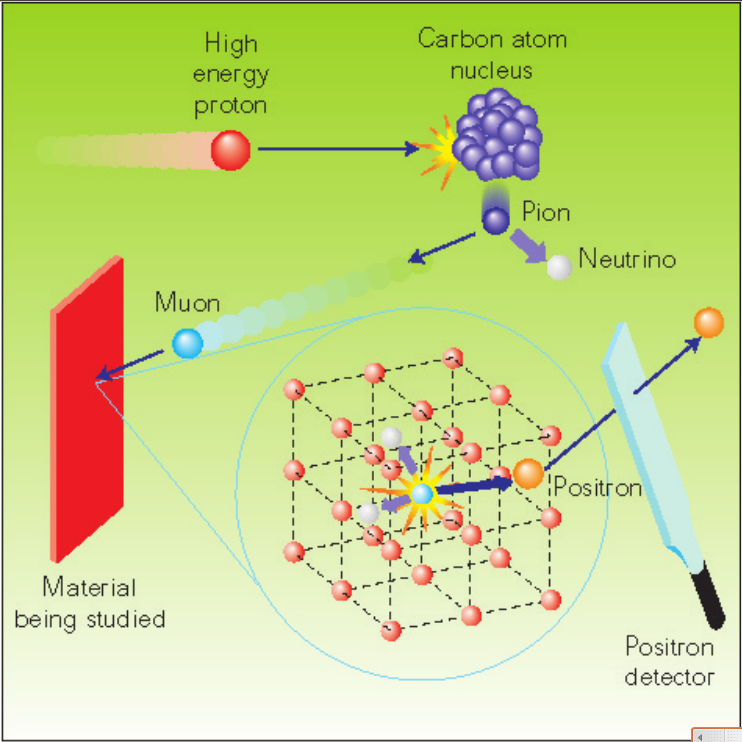
\includegraphics[height=6cm, keepaspectratio]{Bilder/musr_general_principle.png}%
			\caption*{  \setlength{\baselineskip}{6pt}
				{\tiny Dalmas de Réotier, Pierre (2010): \textit{Introduction to muon spin rotation and relaxation (\musr)} [Online]. Availible: \url{http://inac.cea.fr/Pisp/pierre.dalmas-de-				reotier/introduction_muSR.pdf}}
			}%
		\end{center}
	\end{figure}          
\end{frame}






\begin{frame}
	\frametitle{Coexistence of ferromagnetism and superconductivity in RuSr$_2$GdCu$_2$O$_8$}
	
	\begin{columns}
		\column{.55\textwidth}
		\begin{itemize}
			\item ferromagnetic phase is homogenous on a microscopic scale \vspace{10pt}
			\item it accounts for most of the sample volume\vspace{10pt}
			\item magnetic order is not significantly modified at the onset of superconductivity
		\end{itemize}
		\vspace{1cm}
		\vfill
		\setlength{\baselineskip}{6pt}      
		\begin{tiny}
			C. Bernhard, J. L. Tallon, Ch. Niedermayer, Th. Blasius, A. Golnik, E. Brücher, R. K. Kremer, D. R. Noakes, C. E. Stronach, and E. J. Ansaldo, Phys. Rev. \textbf{B} 59, 14099 (1999)
		\end{tiny}
		
		\column{.45\textwidth}
		\begin{figure}[htbp]
			\centering
			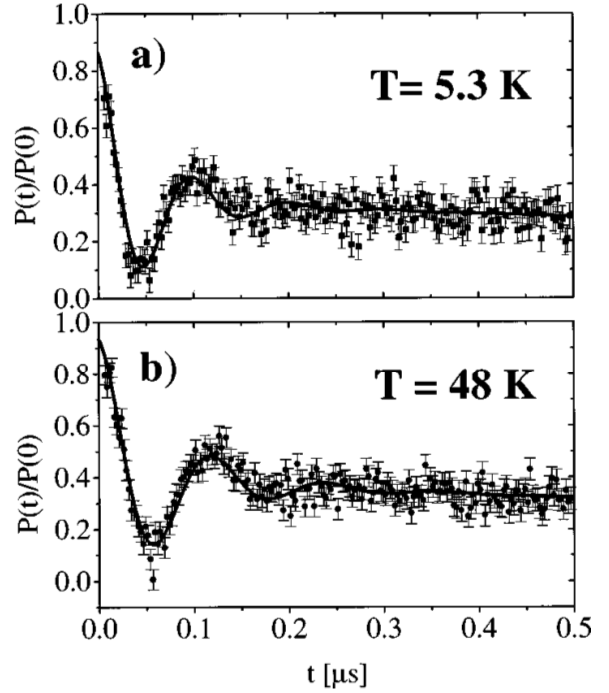
\includegraphics[width=\textwidth]{Bilder/ferromagnetism.png}%
			\caption*{\setlength{\baselineskip}{5pt}{\tiny Time-resolved normalised muon-spin polarisation $^{P(t)}/_{P(t=0)}$ at temperatures $T = 5.3K < T_{c,sc}$ and at $T_{c, sc} < T = 28K < T_{c,m}$ . The large oscillatory component gives clear evidence for the presence of a magnetically ordered state.}}%
		\end{figure}
	\end{columns}
	
	\vfill
	
	
\end{frame}





\begin{frame}
	\begin{columns}
		\column{.45\textwidth}
		\begin{block}{\textbf{5 - 6 }}
			$He$ core is homogenous (convective mixing). It will be nearly isothermal.\\~\\
			
			More and more $He$ is produced by shell burning, the core becomes more massive \\~\\			
			
			At some point, core cannot support envelope mass anymore: \\~\\
			
			
			$\Rightarrow$ core contracts, envelope expands
		\end{block}
		\column{.65\textwidth}
		\vspace{.77cm}
		\pgfimage[width=\textwidth]{Bilder/Scan_Padmanabhan_cropped.pdf}
	\end{columns}	
	\begin{center}
		\fillframe
		\setlength{\baselineskip}{0pt}
		{\tiny
			T. Padmanabhan, "Theoretical Astrophysics Volume II: Stars and Stellar Systems". New York: Cambridge University Press, 2001.
		}
	\end{center}
\end{frame}




\end{document}
